Сбор данных для научных проектов исходя из потребности воспроизводимости эксперимента должен выполняться из открытых источников. 
Такими источниками могут быть книги в общем доступе, олимпиадные задачи и предметные веб-сайты. Также 
сбор данных можно проводить из уже подготовленных научным сообществом корпусов, задавая экспертные критерии
отбора и выполняя перевод с иностранного языка. 

Полученные данные имеют мощность порядка миллиона слов \ref{distribution} 

\begin{figure}[h]
    \centering
    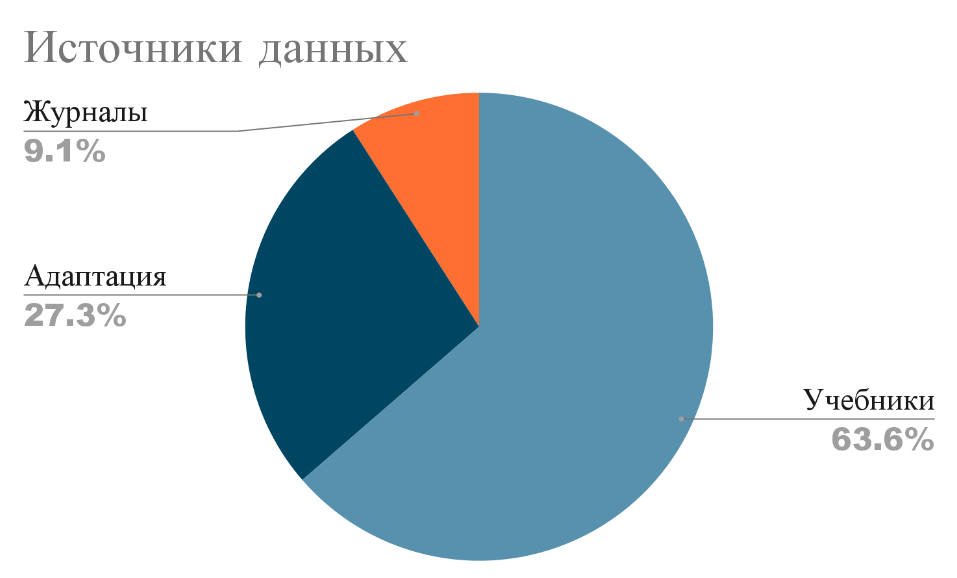
\includegraphics[width=0.5\textwidth]{assets/work/dataset/diagram.png}
    \caption{Распределение данных по источникам.}
    \label{distribution}
\end{figure}

Сбор данных, представленных в виде  документов, не имеющих подготовленного текстового слоя осуществлялся при помощи технологий оптического распознавания символов.
В секции также частично описан метод распознавания, разработанный в рамках данного исследования.

В состав открытого тренировочного набора входит более тысячи аннотированных изображений 

Международные сайты исследователей содержат большое число подготовленных структурированные данных. 
К сожалению, большинство из них представлены на китайском и английский языках. Для их адаптации
предложен подход, использующий большие языковые модели в качестве средств перевода на русский язык.
В работе использовался языковой ассистент llama3, показывающий 
\begin{figure}[h]
    \centering
    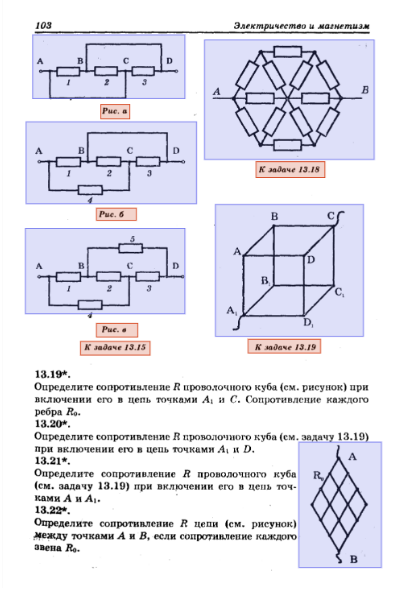
\includegraphics[width=0.5\textwidth]{assets/work/dataset/kirik_labeling.png}
    \caption{Пример аннотированной иллюстрации из книги Генденштейн, Кирик, Гельфгат: 1001 задача по физике.}
    \label{annotation}
\end{figure}

Перевод 7500 задач выполнялся в течении 12 часов. Полученные результаты приведены в предметном репозитории \footnote{\url{https://huggingface.co/datasets/NMashalov/olympiad_task_translation}}
Полный список использованной литературы приведен в приложении к работе \ref{literature}

\begin{figure}[h]
    \centering
    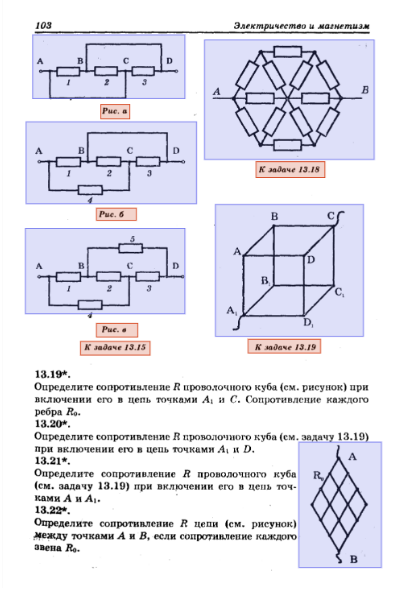
\includegraphics[width=0.5\textwidth]{assets/work/dataset/kirik_labeling.png}
    \caption{Пример аннотированной иллюстрации из книги Генденштейн, Кирик, Гельфгат: 1001 задача по физике.}
    \label{annotation}
\end{figure}

Для адаптации корпуса задач также были подготовлены